\documentclass[conference]{IEEEtran}
\IEEEoverridecommandlockouts
% The preceding line is only needed to identify funding in the first footnote. If that is unneeded, please comment it out.
\usepackage{algorithmic}
\usepackage{amsmath,amssymb,amsfonts}
\usepackage{booktabs}
\usepackage{cite}
\usepackage{hyperref}
\usepackage{graphicx}
\usepackage{lipsum}
\usepackage{tabularx}
\usepackage{textcomp}
\usepackage{xcolor}
\usepackage{subcaption}
\usepackage{systeme}

\def\BibTeX{{\rm B\kern-.05em{\sc i\kern-.025em b}\kern-.08em
    T\kern-.1667em\lower.7ex\hbox{E}\kern-.125emX}}
\begin{document}

\title{RS Paper*\\
{\footnotesize \textsuperscript{*}Note: Sub-titles are not captured in Xplore and
should not be used}
\thanks{Identify applicable funding agency here. If none, delete this.}
}

\author{\IEEEauthorblockN{1\textsuperscript{st} Given Name Surname}
\IEEEauthorblockA{\textit{dept. name of organization (of Aff.)} \\
\textit{name of organization (of Aff.)}\\
City, Country \\
email address}
\and
\IEEEauthorblockN{2\textsuperscript{nd} Given Name Surname}
\IEEEauthorblockA{\textit{dept. name of organization (of Aff.)} \\
\textit{name of organization (of Aff.)}\\
City, Country \\
email address}
\and
\IEEEauthorblockN{3\textsuperscript{rd} Given Name Surname}
\IEEEauthorblockA{\textit{dept. name of organization (of Aff.)} \\
\textit{name of organization (of Aff.)}\\
City, Country \\
email address}
\and
\IEEEauthorblockN{4\textsuperscript{th} Given Name Surname}
\IEEEauthorblockA{\textit{dept. name of organization (of Aff.)} \\
\textit{name of organization (of Aff.)}\\
City, Country \\
email address}
\and
\IEEEauthorblockN{5\textsuperscript{th} Given Name Surname}
\IEEEauthorblockA{\textit{dept. name of organization (of Aff.)} \\
\textit{name of organization (of Aff.)}\\
City, Country \\
email address}
\and
\IEEEauthorblockN{6\textsuperscript{th} Given Name Surname}
\IEEEauthorblockA{\textit{dept. name of organization (of Aff.)} \\
\textit{name of organization (of Aff.)}\\
City, Country \\
email address}
}

\maketitle

\begin{abstract}
Pending.
\end{abstract}

\begin{IEEEkeywords}
pending, pending, pending, pending
\end{IEEEkeywords}

\section{Introduction}
\par In modern communications and storage systems, it is observed the increasingly demand for solutions of high speed data rates and reliability with economic viable hardware. Error Correction Coding (ECC) techniques plays an important role to fulfill these opposite requirements. They aim to incorporate redundancy to the transmitted data and restrict the characteristics of the encoded signal in order to augment the decoder's capability to extract the original data from  unreliable and noisy communication channels \cite{b1}. Reed-Solomon (RS) codes is one of the most popular ECC methods that uses a block-by-block basis to correct burst errors and erasures in data. The adequate compromise between effectiveness and implementation complexity guarantees the widespread use of RS codes in many applications until today.

\par The paper entitled "Polynomial Codes over Certain Finite Fiels" \cite{b2} published in June 1960 was the first formal publication of RS codes. At this time, a pursue to the most optimal and mechanizable ECC emerged after Claude Shannon theory defines the upper bound of the channel capacity at which is possible to transmit error-free information using a proper coding method. Richard Hamming developed the first expressive practical work on ECC algorithms using linear algebra in early 1950s, and then Bose, Ray-Chaudhuri and Hocquenghem generalized his experiments in 1959 - being known as BCH codes. Finally, Irving Reed and Gustave Solomon introduced a special case of BCH codes (RS codes) that employs an efficient decoding algorithm that enabled its wide range use \cite{b3}.

\par Since its introduction, many technologies and standards have adopted RS codes with a variety of parametric configurations. The Compact Disc (CD) system was the first consumer mass application which employed RS codes \cite{b4}, and since then many other used adopted it such as satellite and mobile systems, DVD and barcodes, and digital television. The literature presents many custom hardware implementations of RS Codecs even though they only differs in parametric terms. Current Hardware Description Languages (HDL) - Verilog and VHDL - already provide ways to express a parametric Register Transfer Level (RTL) architecture; however, it has not been completely explored in previous works. Also, verification of generic RTL blocks might be challenging and requires a proper methodology to assess implementation against block requirements. Most papers that explore RS codecs only provide a limited validation of the RTL implementation without analyzing metrics and results that certifies the block verification.  

\par This work proposes a generic RTL implementation in VHDL and verification of a RS codec. The primary goal of this study is to present an open access IP of a RS codec that could be used as baseline for future works, and not to provide an optimized RTL architecture of it. The block will be verified by using Formal Verification (FV) approach, which is an emerging technology that has been becoming widely adopted in IP designs. Verifying all parametric combinations would not be feasible - or even impossible -, then this paper will use IEEE 802 standard as background. The IEEE 802 group, which develops standards and recommended practices for local, metropolitan, and other area networks, catalogs many commercial RS codec specifications with a diverse range of parametric setups that will be explored in this work.     

\par The paper is organized as in the following: Section II introduces theoretical aspects of RS codes, section III analyzes related works, section IV presents the proposed RTL architecture of the RS codec, section V examines and exhibits results of the adopted verification approach, section VI explores synthesis aspects of the implemented IP and the paper conclusion is presented in section VII.

\section{Reed-Solomon Codes: Theoretical Aspects}

\par What are RS codes? This fundamental question can be the starting point for discussing the theory behind it. The authors of RS codes  already answered it using few lines in \cite{b5}:

\begin{quote}
``They are simply sets of algebraic curves defined by polynomials with a limited range of degrees. These curves when graphed are a set of discrete points - the abscissas and ordinates are values in a Galois Field (GF). The degree limitation allows recovery of the complete curve even when the graph is assumed to be smudged and erased at many points. The relation of this idea to error control on noise-corrupted digital communication channels is immediate.''
\end{quote}

\par Even without knowing GF, it is possible to have a glimpse of how RS codes work. It basically relies on "fitting" points in a plane by the polynomial of smallest degree that passes through these points \cite{b6}. Basic polynomial mathematics affirms that 2 points can be fitted by a straight line, 3 points by a parabola, and so on. If some redundancy is added by oversampling a given polynomial function, the curve can be correctly guessed even though some recorded points move unintentionally. For instance, assuming that a parabola, which can be represented by $k = 3$ points, is recorded in $n = 7$ points (\hyperref[fig:fig1a]{Fig. 1a}). If $t = 2$ points are moved vertically, the original polynomial can still be recovered by finding a single parabola that fits as many as possible of the 7 points (\hyperref[fig:fig1b]{Fig. 1b}). 
%TODO: Check figure reference. It is not showing a and b. Maybe this is nohow it should be done.

%\begin{figure}[!hbt]
%  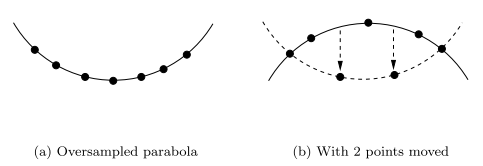
\includegraphics[width=\linewidth]{figures/fig1.png}
%  \caption{Example with $n = 7$ and $k = 3$.}
%  %TODO: This image is copy and paste!
%  \label{fig:fig1}
%\end{figure}

\begin{figure}[!hbt]
  \begin{subfigure}[b]{0.45\columnwidth}
    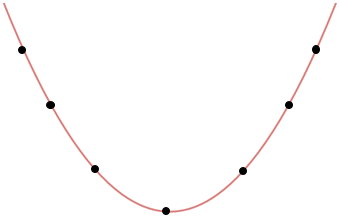
\includegraphics[width=\linewidth]{figures/fig1_a.png}
    \caption{}
    \label{fig:fig1a}
  \end{subfigure}
  \hfill %%
  \begin{subfigure}[b]{0.45\columnwidth}
    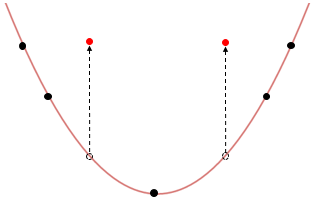
\includegraphics[width=\linewidth]{figures/fig1_b.png}
    \caption{}
    \label{fig:fig1b}
  \end{subfigure}
  \caption{Parabola sampled in $n=7$ points (a). The same parabola is still recovered even though two recorded points are erroneously moved (b).}
\end{figure}

\par It is known that if $t$ is greater than half of the number of extra points, an incorrect polynomial function may fit the greatest number of points. Therefore, $t = (n - k)/2$ represents the maximum capacity of error correction. RS codes can be seen in such way, but applied in the universe of field arithmetic. Therefore, RS codes are represented as a set of length $n$ vectors (codewords) where their elements (symbols) consist of $q$ binary digits (\hyperref[fig:fig2]{Fig. 2}). The original message takes $k$ vector positions, then there are $n-k$ redundant symbols (parity). A RS codec configuration is usually referred by the notation RS$(n, k)$.    

\begin{figure}[!hbt]
  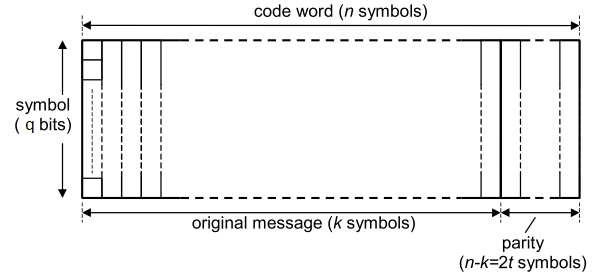
\includegraphics[width=\linewidth]{figures/fig2.png}
  \caption{Generic parametric configuration of RS codes (figure adapted from Fig.1s in \cite{b8}).}
  \label{fig:fig2}
\end{figure}  

\par RS codes are linear, all codewords are sums of codewords, and cyclic, every cyclic shift of a code word is also a codeword \cite{b8}. These properties make the hardware implementation of the codec feasible, and this is granted only because of the application of GF during encoding and decoding processes. Its algebra establishes restricted rules in a finite field, thus every arithmetical operation will result in an element within a finite number of elements. GF is built using a primitive element $\alpha$ which is root of a primitive polynomial ($p(x)$) used as reference to generate the field elements. For digital world it is convenient to choose $\alpha = 2$ since it represents the binary notation. Hence, the total number of elements in a GF corresponds to $2^q$. \hyperref[tab:t1]{Table 1} is a example of GF($2^3$) where $\alpha = 2$ is root of $p(x)$. Hence, $\alpha^3 + \alpha + 1 = 0$, or equivalently $\alpha^3 =  \alpha + 1$ (additions and subtractions are interchangeable in field arithmetic).

\begin{table}[!hbt]
\captionsetup{justification=centering, labelsep=newline}
\centering
\label{tab:t1}
\caption{GF($2^3$) representation using $p(x) = x^3 + x + 1$ } 
%\begin{tabular}{lcl}
\begin{tabular}{ccc}
\toprule
Index Form  & Polynomial Form & Decimal Form                                                                                                    \\
\midrule
$0$ & $0$ & $0$                                                                                              \\
$\alpha^0$ & $1$ & $1$                                                                                         \\
$\alpha^1$ & $\alpha$ & $2$
\\
$\alpha^2$ & $\alpha^2$ & $4$                                                                                        
\\
$\alpha^3$ & $\alpha + 1$ & $3$                                                                                        
\\
$\alpha^4$ & $\alpha^2 + \alpha$ & $6$                                                                                        
\\
$\alpha^5$ & $\alpha^2 + \alpha + 1$ & $7$                                                                                        
\\
$\alpha^6$ & $\alpha^2 + 1$ & $5$                                                                                        
\\
\bottomrule
\end{tabular}
\end{table}

\par The approach to generate RS codes published in the original paper \cite{b2} takes a sequence of symbol information, $\{m_{k - 1}, m_{k - 2}, ..., m_1, m_0\}$, to build the polynomial $M(x) = m_{k-1}x^{k-1} + m_{k-2}x^{k-2} + ... + m_{1}x + m_0$. If $n \leq \alpha^m$ elements from GF($\alpha^m$) are evaluated in $M(x)$, then the result is a system of $n$ linear equations in $k$ variables \eqref{eq:1}. This system can be solved using any $n \choose k$ combinations of equations. If the number of corrupted symbols $t \leq (n - k)/2$, the most occurring solution of $n \choose k$ linear systems corresponds the original message. However, this method clearly requires much computational resources to calculate all possible solutions.  

\begin{equation}
\label{eq:1}
\begin{aligned}
& \scriptscriptstyle M(0)=m_0 \\
& \scriptscriptstyle M(\alpha)=m_{k-1}\alpha^{k-1} + ... + m_{2}\alpha^{2} + m_1\alpha + m_0 \\
& \scriptscriptstyle M(\alpha^2)=m_{k-1}\alpha^{2(k-1)} + ... + m_{2}\alpha^{4} + m_1\alpha^{2} + m_0   \\
& \scriptscriptstyle ...\\
& \scriptscriptstyle M(\alpha^{2^m-1})=m_{k-1}\alpha^{(2^m-1)(k-1)} + ... + m_{2}\alpha^{(2^m-1)2} + m_1\alpha^{(2^m-1)} + m_0
\end{aligned}
\end{equation}

\par The most practical approach uses Generator Polynomials (GP) \eqref{eq:2} for codification. The roots of GP are composed by $2t - 1$ consecutive elements of the adopted GF. Usually, $b$ is chosen to be 0. It can be demonstrated that cyclic codes can always be defined by a GP \cite{b3}, which implies that the resulting codeword contains coefficients of a polynomial that is divisible by the GF. This assumption culminates in a more efficient implementation for RS codec \cite{b9}. The next topics describe encoding and decoding processes of RS codes using GPs.

\begin{align}
\label{eq:2}
\begin{gathered}
G(x) = (x + \alpha^b)(x + \alpha^{b + 1})...(x + \alpha^{b + 2t-1})
\end{gathered}
\end{align}
%most common case

\subsection{Encoding Process} \label{encoding_process}

\par The encoding process exploits the polynomial division of $M(x)$ by $G(x)$ in a GF($\alpha^q$), as demonstrated by \eqref{eq:3}. $M(x)$ shifted by $n - k$ positions (multiplication by $x^{n - k}$) in order to reserve the lowest $n - k$ positions to the parity check symbols. $Q(x)$ and $R(x)$ are the quotient and the remainder of the division operation. If  $\{m_{k - 1}, m_{k - 2}, ..., m_1, m_0\}$ is assigned to be the first $k$ elements of the codeword that forms $C(x)$, then the coefficients of $R(x)$ are the appropriate elements to shape $C(x)$ in such way that it is divisible by $G(x)$. Equation \eqref{eq:4} shows the result of the encoding process.

\begin{align}
\label{eq:3}
\begin{gathered}
\frac{x^{n - k}M(x)}{G(x)}  = Q(x)G(x) + R(x)
\end{gathered}
\end{align}

\begin{equation}
\label{eq:4}
\begin{aligned}
& C(x)\ =\ x^{n - k}M(x) + R(x)\\
& \ \ \ \ \ \ \ =\ m_{k-1}x^{n-1} + ... + m_0x^{n-k} \\
& \ \ \ \ \ \ \ \ \ \ \ + r_{n-k-1}x^{n-k-1}+...+r_0
\end{aligned}
\end{equation}

\subsection{Decoding Process} 

	\par Errors might be added to $C(x)$ during a codeword transmission through a channel, and $E(x)$ corresponds to the polynomial defined by the errors introduced into the encoded codeword. Then, the received codeword $R(x)$ is the sum between $C(x)$ and $E(x)$. The number of non-zero coefficients of $E(x)$ must be less than $(n - k)/2$ for obtaining original message after decoding $R(x)$. The following sequential steps are required for the decoding process:
	
\begin{itemize}
	\item Compute syndrome terms
	\item Calculate the coefficients of the error-location polynomial $\sigma (x)$
	\item Find the locations of the errors
	\item Find the values of the errors
	\item Correct $R(x)$ given error locations and values 
\end{itemize}
\hfill \break
\subsubsection{Syndrome Calculator}
\par The syndrome characterizes a particular error pattern in the received codeword. It generates the polynomial $S(x)$ \eqref{eq:5}, which is reference for next steps. If $S(x) = 0$, $R(x)$ is error free. 

\begin{align}
\label{eq:5}
\begin{gathered}
S(x) = \sum_{i=b}^{b+2t-1}S_{i}x^{i-b}, \ where\ S_i = R(\alpha^i)
\end{gathered}
\end{align}

The computation of each coefficient $S_i$ of $S(x)$ 


\begin{itemize}
	\item Principle
	\item Algorithm
\end{itemize}
\subsubsection{Euclidean}
\begin{itemize}
	\item Principle
	\item Algorithm
\end{itemize}
\subsubsection{Chien Search}
\begin{itemize}
	\item Principle
	\item Algorithm
\end{itemize}
\subsubsection{Forney}
\begin{itemize}
	\item Principle
	\item Algorithm
\end{itemize}
\subsection{RS in IEEE 802}
\par The IEEE 802 specifies Local Area Network (LAN) and Metropolitan Area Network (MAN) standards and is mainly focused on the Medium Access Control (MAC) and Physical (PHY) layers of the ISO Reference Model for Open Systems Interconnection (OSI). The whole standardization process is coordinated by IEEE 802 LAN/MAN committee, and its first meeting was held in February of 1980. IEEE-802 LMSC is organized into a number of Working Groups (WGs) and Technical Advisory Groups (TAGs) operating under the supervision of a sponsor Executive Committee (EC) \cite{b10}. The current active IEEE802 WGs/TAGs are listed below:

\begin{itemize}
\item 802.1: Higher Layer LAN Protocols
\item 802.3: Ethernet 
\item 802.11: Wireless LAN
\item 802.15: Wireless Personal Area Network (PAN)
\item 802.18: Radio Regulatory
\item 802.19: Wireless Coexistence
\item 802.21: Media Independent Handover Services
\item 802.22: Wireless Regional Area Networks
\item 802.24: Vertical Applications
\end{itemize}

The IEEE 802 standards that rules PHY layers establishes many procedures to guarantee the minimal requirements for communication systems in a given application scenario. RS codecs are defined in many sub-items of the IEEE 802 standards, and \hyperref[tab:t1]{Table II} enumerates their main occurrences. It demonstrates how varied are the parametric definitions for RS codecs.
%And the need for hardware implementation?

\begin{table}[!hbt]
\captionsetup{justification=centering, labelsep=newline}
\centering
\label{tab:t2}
\caption{Parametric configurations of RS codecs in IEEE 802} 
%\begin{tabular}{lcl}
\begin{tabular}{ccc}
\toprule
Standard  & Interfaces & RS Config.                                                                                                    \\
\midrule
IEEE 802.3 & D-PSK symbols & RS(15,11)
\\
IEEE 802.3 & 10PASS-TS & RS(144,128)
\\
IEEE 802.3 & 25GBASE-SR & RS(192,186)
\\
IEEE 802.3 & ITU-T G.975 & RS(255,239)
\\
IEEE 802.3 & 10GBASE PR-D, PR-U, and PRX-U & RS(255,223)
\\
IEEE 802.3 & 1000BASE-T1 & RS(450,406)
\\
IEEE 802.3 & 25GBASE-R & RS(528,514)
\\
IEEE 802.3 & 100GBASE CR4, KR4, and SR4 & RS(528,514)
\\
IEEE 802.3 & 100GBASE-KP4 & RS(544,514)
\\
IEEE 802.3 & 200GBASE-R & RS(544,514)
\\
IEEE 802.3 & 400GBASE-R & RS(544,514)
\\
IEEE 802.11 & PHY & RS(204,208)
\\
IEEE 802.15.3 & SC PHY & RS(255,239)
\\
IEEE 802.15.3c & THz-OOK PHY MCS 1 & RS(15,11)
\\
IEEE 802.15.3c & THz-OOK PHY MCS 2 & RS(15,14)
\\
IEEE 802.15.3c & THz-OOK PHY MCS 0 & RS(240,224)
\\
IEEE 802.15.7 & - & RS()
\\
IEEE 802.15.7 & PHY I - OOK 11.67 kb/s or VPPM 124.4 kb/s & RS(15,7)
\\
IEEE 802.15.7 & PHY I - OOK 24.44 kb/s & RS(15,11)
\\
IEEE 802.15.7 & PHY I - VPPM 35.56 kb/s & RS(15,2)
\\
IEEE 802.15.7 & PYH I - VPPM 71.11 kb/s & RS(15, 4)
\\
IEEE 802.15.7 & PHY II & RS(64,32)
\\
IEEE 802.15.7 & PHY II and III & RS(160,128)
\\
\bottomrule
\end{tabular}
\end{table}

The choose of $n$ depends on the intended data rate of the related interface. For the number of data symbols $k$, the expected channel characteristics such as noise and bandwidth and the required reliability level dictates its values.\hyperref[fig:fig31]{Fig. 3} illustrate the relation between Bit Error Rate (BER) and Energy per Bit to Noise Power Spectral Density Ratio ($E_{b}/N_{0}$) for  different RS codec configurations. It resulted from a transmission simulation using Pulse-Amplitude Modulation with 16 discrete levels (PAM-16) sent over a Additive White Gaussian Noise (AWGN) channel. 


\begin{figure}[!hbt]
  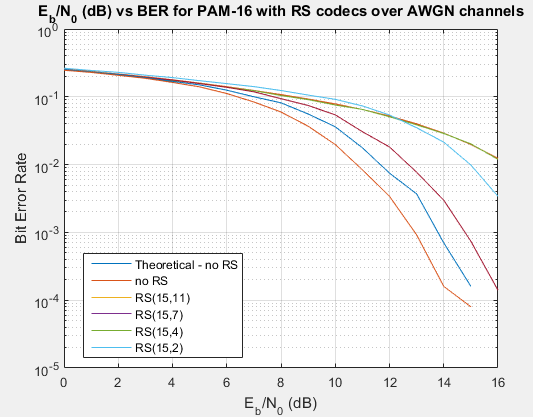
\includegraphics[width=\linewidth]{figures/fig_13.png}
  \caption{Transmission efficiency for PAM-16 over AWGN channels using RS codecs with $n = 15$ and $k = 11, 7, 4, 2.$}
  \label{fig:fig31}
\end{figure}  

\section{RS Codes: RTL Design}

Add one generic paragraph
\subsection{Encoder}

According to \ref{encoding_process}, the encoded codeword consists of the own input data symbols and the result of the $mod$ operation between $x^{n - k}M(x)$ and $G(x)$. Besides that, it is required a proper module interface that enables coordination of control operations such as informing starting and ending of codewords, data validity and other aspects. \hyperref[tab:t2]{Table 2} describes all RS Encoder ports. 

\begin{table}[!hbt]
\label{tab:t2}
\caption{RS Encoder ports}
\begin{tabular}{lcl}
\toprule
Name               & I/O & Description                                                                                                    \\
\midrule
clk                & I   & System clock pin                                                                                               \\
rst                & I   & System reset pin                                                                                               \\
i\_start\_codeword & I   & Indication of input codeword start                                                                             \\
i\_end\_codeword   & I   & Indication of input codeword end                                                                               \\
i\_valid           & I   & Validity of input symbols and indicators                                                                   \\
i\_symbol          & I   & Input data symbol                                                                                              \\
o\_start\_codeword & O   & Indication of output codeword start                                                                            \\
o\_end\_codeword   & O   & Indication of output codeword end                                                                              \\
o\_in\_ready       & O   & Ready to accept input symbols and indicators\\
o\_valid           & O   & Validity of output symbols and indicators                                                                  \\
o\_error           & O   & Unexpected behavior happened                                                                                   \\
o\_symbol          & O   & Output data symbol                                                                                            
\\
\bottomrule
\end{tabular}
\end{table}

The top level architecture has control and processing units as seen in \hyperref[fig:fig4]{Fig. 3}. The processing unit is only responsible for computing the $mod$ operation and output the encoded symbols. It is managed by the control unit, which initializes and interrupts the processing unit and outputs reference signals. Also, input symbols are delayed by one cycle as the control unit requires such delay to know which action should be done with the input symbol. There is an output register as well responsible for synchronizing all output signals of the RS Encoder. The only exception is o\_in\_ready because a readily response is required for this signal, which is a reference to blocks that drives RS Encoder inputs.

\begin{figure}[!hbt]
  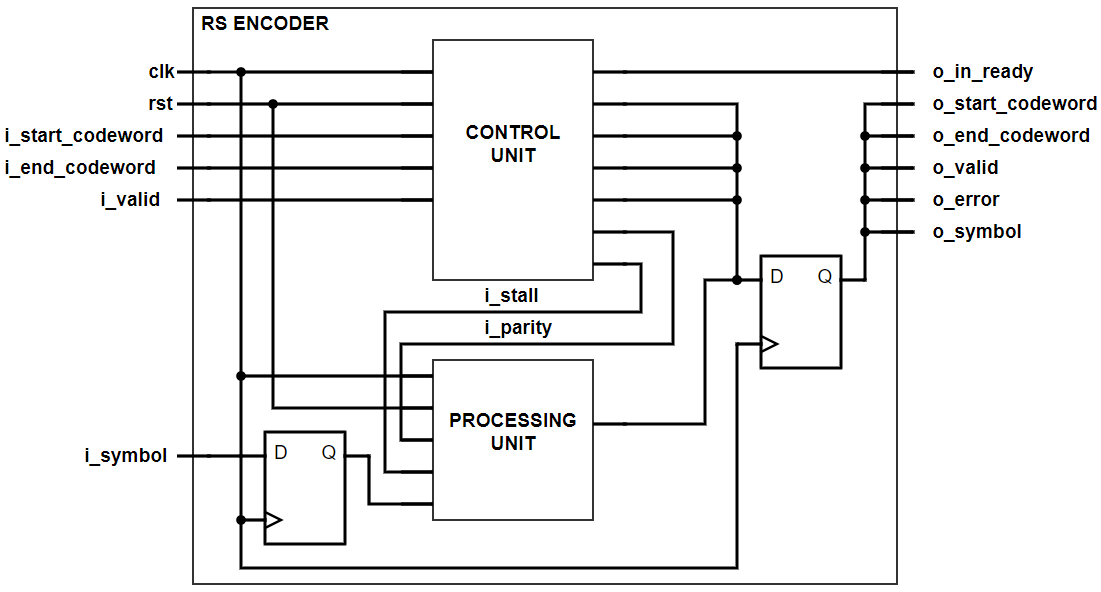
\includegraphics[width=\linewidth]{figures/fig5.png}
  \caption{Top level architecture for RS Encoder.}
  \label{fig:fig4}
\end{figure}  

\begin{figure*}
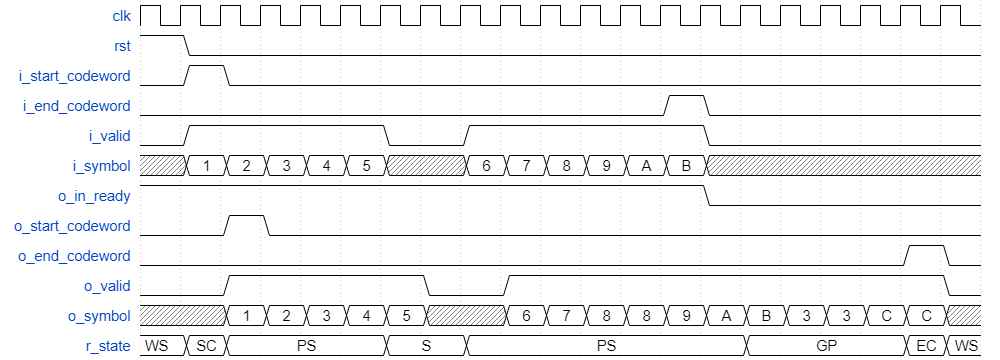
\includegraphics[width=\textwidth,height=5cm]{figures/fig4.png}
  \caption{Waveform example of the encoding process in GF($2^4$) }
  %TODO: This image is copy and paste!
  \label{fig:fig5}
\end{figure*} 

\subsubsection{Processing Unit}
%recap generator polinomial
The $mod$ operation can be performed by a Linear Feedback Shifter Register (LFSR). The remainder is incrementally computed for the first $k$ input symbols, which represents the coefficients of $C(x)$ starting from the highest order. The depth of the LFSR corresponds to the number of parity symbols, which is $n$ - $k$. \hyperref[fig:fig6]{Fig. 6} shows the schematic of the Processing Unit. Originally, subtractions are required during the calculation of the reminder, but sum is equivalent to subtraction in GF. The GF adder A\_div is responsible for finding the quotient term. This number is multiplied by the GP coefficients, with the exception of the highest ($x^{2t}$ according to equation \ref{eq:2}) that was already canceled in the current division operation step. The multiplication result is them summed (or subtracted) with the previous terms and stored into the registers. After $k$ steps, the remainder result is completed, and then it can be output by selecting the first input of the output mux (M\_out). Every register has a mux in its data input that may conserve its state when the $mod$ calculation is interrupted.  

%https://www.digikey.com/schemeit/project/newproject-1-ETEUM584030G/

\begin{figure}[!hbt]
  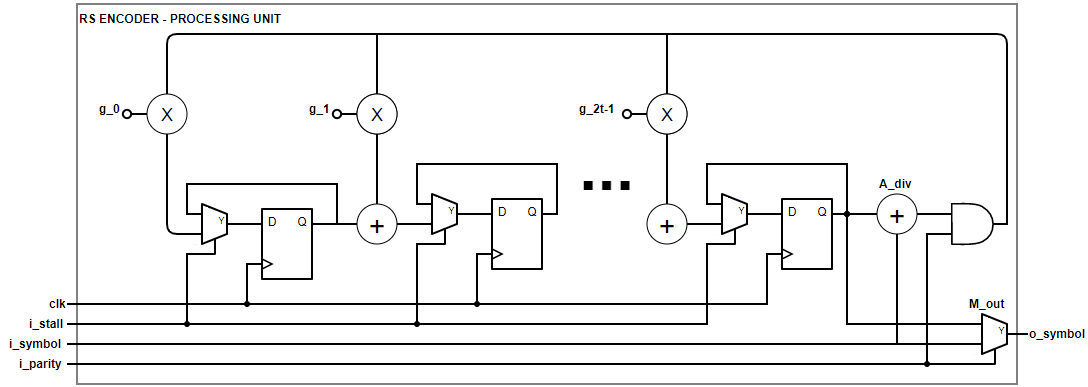
\includegraphics[width=\linewidth]{figures/fig12_a.png}
  \caption{Design implementation of Processing Unit}
  %TODO: This image is copy and paste!
  \label{fig:fig6}
\end{figure}  

\subsubsection{Control Unit}
The Control Unit implements the Finite State Machine (FSM) showed in \hyperref[fig:fig7]{Fig. 7}. WAIT\_SYMBOL (WS) is the initial state and looks for the first valid input symbol. Once it is found, the next state is START\_CODEWORD (SC), which enables the Processing Unit to receive the sequence symbols to be encoded and also asserts o\_start\_cw for $1$ cycle. Then, PROCESS\_SYMBOLS (PS) takes over and supervises the input symbols until the input message ending, signaled by i\_end\_cw. The transition condition is related to $r\_cnt$, which is a counter that indicates how many symbols were processed. When it reaches the maximum number of allowed input symbols (MAX\_I\_SYM) having a previous i\_end\_cw signaling, the FSM is ready to go to GENERATE\_PARITY (GP). This state is responsible for controlling the output of parity symbols stored into the registers of the Processing Unit. $r\_cnt$ is incremented each cycle until it is equal to NUM\_SYM, which means that all parity symbols were outputted. Finally, the Control Unit will return to WS or SC, depending on whether a new message is available or not. STALL and ERROR states are related to interruptions and unexpected behaviors. Whenever i\_valid is de-asserted during input message reception (SC and PS), STALL state assumes to freeze the Processing Unit until i\_valid is re-enabled. The ERROR state is reached when i\_start\_cw and i\_end\_cw assume unexpected values at a given state (refereed by \*unexpected\* in \hyperref[fig:fig7]{Fig. 7}). Once ERROR state is reached, it is required to reset the RS Encoder. 

%Whenever i\_valid is de-asserted during input message reception, STALL state assumes util i\_valid is re-enabled, and the Processing Unit is interrupted.

%$ If $i_valid$ is disabled, $STALL$ is hit, and it remains there until $i\_valid$ is re-enabled. $r\_cnt$ is a counter that indicates how many input symbols were processed, and reference for PS state transition. The condition for transition is when it reaches the maximum number of allowed input symbols ($MAX\_I\SY$). There is also an ERROR state, which indicates that some invalid behavior happened during during the encoding process. Examples are multiple i_start_cw or i_end_cw pulses and missing i_end_cw during the life time of the PS state. Once ERROR is reached, only rst can leave from there.  

% Once this condition is reached, the Process Unit is activated for receiving the message to be encoded. This state is represented by 
%Control is a state machined with states figura wit bla First i_start_code, processing. receives and monitor the validy o ht signal. If its is invalid it goes to stall - it remains there until valid in 1 again. When all message is processed.. the remainder is formed and outputed. EC is the last coddeowrd. Then the is cycle starts again. Also, there is a error state which when some wrong scenario happen such as receiving start_cod and end_cov unexpectly. Once is error, only a hard reset makes it to go to wait.The figure show the waveform, endocing, all states. The states looks early because the output is delayed by one cycle. 

\begin{figure}[!hbt]
  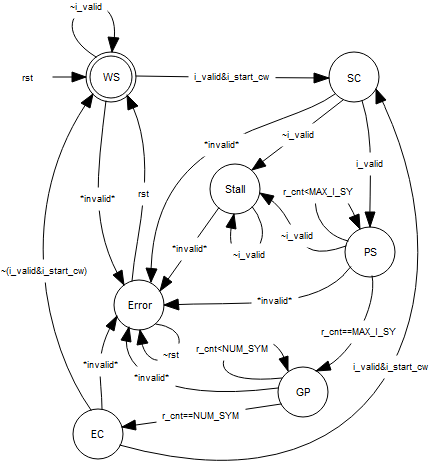
\includegraphics[width=\linewidth]{figures/fig10.png}
  \caption{FSM designed in Control Unit}
  %TODO: This image is copy and paste!
  \label{fig:fig7}
\end{figure}  

\subsection{RS Decoder}
\begin{itemize}
	\item Interface and explain how it works. Show waveform example for the most common operator conditions. Use https://wavedrom.com/ for it - no print screens from simulator waveform visualizer.
	\item Diagram with architecture and explanation
\end{itemize}
\subsubsection{Syndrome}
\begin{itemize}
	\item Architecture
	\item State Machine
\end{itemize}
\subsubsection{Euclidean}
\begin{itemize}
	\item Architecture
	\item State Machine
\end{itemize}
\subsubsection{Chien Search}
\begin{itemize}
	\item Architecture
	\item State Machine
\end{itemize}
\subsubsection{Forney}
\begin{itemize}
	\item Architecture
	\item State Machine
\end{itemize} 
 \subsubsection{FIFOS}
\begin{itemize}
	\item Calculation of FIFO size
\end{itemize} 
 
\section{REED SOLOMON - Verification}
\begin{itemize}
	\item Explain the challenges of verifying a generic RTL. Introduce formal verification and explain why it fits this problem. 
	\item Methodology. Use this reference: A Coverage-Driven Formal Methodology for Verification Sign-off \end{itemize}

\subsection{RS Encoder}
\begin{itemize}
	\item Testplan
	\item Formal test bench arch.
	\item Results
\end{itemize}

\subsection{RS Decoder}
\begin{itemize}
	\item Testplan
	\item Formal test bench arch.
	\item Results
\end{itemize}

\subsection{Verification bug tracking}
Show plots about number of bugs found and time.

\subsection{Formal effort analysis}
The idea here is show how formal verification scales (or not) with more complex RS configurations


\section{REED SOLOMON - Synthesis}
\begin{itemize}
	\item Estimation of Area and number of gates. Here we can compare our IP with commercial IPs.
	\item Synthesis report
	\item Critical path and maximum clock
\end{itemize}

\section{REED SOLOMON - Implementation details}
\begin{itemize}
	\item show the vhdl file structure and tests
	\item Explain pyhton script for generating constants
\end{itemize}

\section{REED SOLOMON - Conclusion}
...

\section*{Acknowledgment}

The preferred spelling of the word ``acknowledgment'' in America is without 
an ``e'' after the ``g''. Avoid the stilted expression ``one of us (R. B. 
G.) thanks $\ldots$''. Instead, try ``R. B. G. thanks$\ldots$''. Put sponsor 
acknowledgments in the unnumbered footnote on the first page.

\section*{References}

Please number citations consecutively within brackets \cite{b1}. The 
sentence punctuation follows the bracket \cite{b2}. Refer simply to the reference 
number, as in \cite{b3}---do not use ``Ref. \cite{b3}'' or ``reference \cite{b3}'' except at 
the beginning of a sentence: ``Reference \cite{b3} was the first $\ldots$''

Number footnotes separately in superscripts. Place the actual footnote at 
the bottom of the column in which it was cited. Do not put footnotes in the 
abstract or reference list. Use letters for table footnotes.

Unless there are six authors or more give all authors' names; do not use 
``et al.''. Papers that have not been published, even if they have been 
submitted for publication, should be cited as ``unpublished'' \cite{b4}. Papers 
that have been accepted for publication should be cited as ``in press'' \cite{b5}. 
Capitalize only the first word in a paper title, except for proper nouns and 
element symbols.

For papers published in translation journals, please give the English 
citation first, followed by the original foreign-language citation \cite{b6}.

\begin{thebibliography}{00}
%http://engineeringjournals.stmjournals.in/index.php/CTSP/article/view/2193
%Esse artigo foi o ultimo lancado
\bibitem{b1} Geisel, William A. "Tutorial on Reed-Solomon error correction coding." (1990)
%Found in page 3
\bibitem{b2} Reed, Irving S., and Gustave Solomon. "Polynomial codes over certain finite fields." Journal of the society for industrial and applied mathematics 8.2 (1960): 300-304.
\bibitem{b3} Stephen B. Wicker; Vijay K. Bhargava., (1994) “An Introduction to Reed-Solomon Codes,” Prentice-Hall
%chapter 1
\bibitem{b4} KAS Immink, ''Reed-Solomon Codes and the Compact Disc'' in SB Wicker and VK
Bhargava, Eds., Reed-Solomon Codes and Their Applications, IEEE Press, 1994.
\bibitem{b5} Reed, Irving S., and Gustave Solomon. ''Reed-Solomon Codes: A Historical Overview'' in SB Wicker and VK Bhargava, Eds., Reed-Solomon Codes and Their Applications, IEEE Press, 1994.
\bibitem{b6} Jack Keil Wolf, “An Introduction to Reed-Solomon Codes”, www.ece.tamu.edu/~hpfister/courses/ecen604/rspoly.pdf.
\bibitem{b7} M. Young, The Technical Writer's Handbook. Mill Valley, CA: University Science, 1989.
\bibitem{b8} Clarke, C. K. P. "Reed-Solomon error correction." BBC R\&D White Paper, WHP 31 (2002).
\bibitem{b9} See link below 
%"https://www2.cs.duke.edu/courses/spring10/cps296.3/rs_scribe.pdf"
\bibitem{b10} IEEE, “Overview and Guide to the IEEE 802 LMSC,” IEEE,
Tech. Rep., Mar. 2008. [Online]. Available: http://ieee802.org/
IEEE-802-LMSC-Overview-and-Guide-01.pdf
\end{thebibliography}

\vspace{12pt}
\color{red}
IEEE conference templates contain guidance text for composing and formatting conference papers. Please ensure that all template text is removed from your conference paper prior to submission to the conference. Failure to remove the template text from your paper may result in your paper not being published.

\end{document}
